\chapter{引言}\label{chap:introduction}

\section{本文的研究背景与意义}

% 问题 -> 
% - 数据中心规模不断扩大
% - 提升利用率的重要性
% 解决方式 -> 混部技术
% - LS 和 BE 应用天然具备混部
% - 通过混部的确解决了问题
% 局限 -> QOS
% 本质 -> 混部共享资源的竞争
% - CPU\Cache\Memory\IO\Net
% - AVX
% 研究现状
% - 劣化监测
% - 调度
% 本研究

云计算为用户提供了使用计算资源的便捷方式,同时虚拟化技术让云计算服务具备了弹性、安全等特征,能够大大减轻服务上云的管理负担。而随着Podman、Docker等容器技术的发展,服务上云的门槛也被极大降低,同时,随K8s、OpenShift等容器编排技术发展及DevOps概念的推广,使得企业与普通用户都越来越倾向于服务上云。不断扩张的需求催生了巨大的云计算市场,这也促使着云厂商不断扩大着数据中心的规模,据中国信息通信研究院的中国算力发展指数白皮书(2023年)显示,2022年国内基础算力规模达到180EFlops,位居全球第二,同时在用数据中心机架规模超过650万个标准机架\citep{chinaict2023}。

庞大的数据中心带来了巨大的管理治理挑战。微软Azure是世界最大的云厂商之一,其调研内部数据发现在数据中心中,每提升1\%的利用率,能够每年节省近1亿美元\citep{hadary2020protean}。因此,如何高效地利用数据中心海量的计算资源,提高整体资源利用率是云厂商重点的关注的核心问题。

超卖是云厂商提升数据中心资源利用率的一种方式,主要涉及到计算资源与存储资源。CPU超卖是最常见的计算资源超卖方式,虚拟化技术让同一个物理CPU上能够运行多个vCPU,存储池化技术则使得云厂商能够出售用户比实际存储还要多的存储资源。随虚拟化技术的不断发展,一方面,虚拟化开销在不断降低,另一方面,虚拟化层次也在不断提升。更高的虚拟化层次模糊了用户的计算需求,为云厂商进行超卖提提供了更多的空间。然而越来越极限的超卖比无疑会造成更激烈的资源竞争,从而导致严重的用户服务质量(QoS)下降,这对云厂商而言意味用户数量的流失。

考虑到服务器上越来越丰富的计算资源能够支持更多的应用同时运行,混部技术逐渐成为当前云厂商提升数据中心利用率的主要方式。混部同样能够将更多的任务调度到同一个服务器上,但不同于资源超卖,混部考虑了数据中心所部署应用的互补特征。当前数据中心应用依据用户对延迟的敏感度,可划分为延迟敏感性(LC)与尽力交付型(BE),前者通常为交互型应用,如在线购物等,用户对于延迟要求较高,后者则通常为离线应用,如大数据处理等。以阿里云为例,通过混部分别将集群的平均CPU利用率和内存资源利用率提升到了38.2\%和88.2\%\citep{guo2019limits}。

然而混部并没有解决资源竞争导致用户QoS劣化的问题。一方面,服务器整体处理能力有限,无论资源超卖还是混部,都试图向单一服务器上引入更多的任务,来挖掘资源利用的极限,而过多的任务就会积压导致排队,从而产生较大的延迟。另一方面,服务器局部的硬件资源也容易成为瓶颈,常见混部策略试图让延迟敏感度不同的应用同时运行,然而数据中心软件环境较为复杂,不同应用也有不同的资源敏感度,同时运行的应用就容易因某一处共享的资源上的激烈竞争导致严重的性能劣化。

竞争本质是共享资源的供小于求,因此分析竞争问题首先需要了解服务器上的共享资源。调度域(Scheduler Domains)\citep{schedulerdomains}在Linux 2.6中首次引入,用来对当时逐渐流行的多核处理上的调度进行协助,而随着CPU设计与制造的不断进步,CPU的拓扑结构也越来越复杂,如超线程技术(Hyperthreading)、非同一内存访问架构(NUMA)、大小核心架构等,CPU架构上的新特性给Linux调度带来的巨大的挑战,如图~\ref{fig:scheduling_domain}所示,调度域作为应对这一挑战的关键抽象层,提供了一种机制,使得Linux内核能够更好地理解CPU之间的关系,从而更智能地进行任务调度。

\begin{figure}[!htbp]
    \centering
    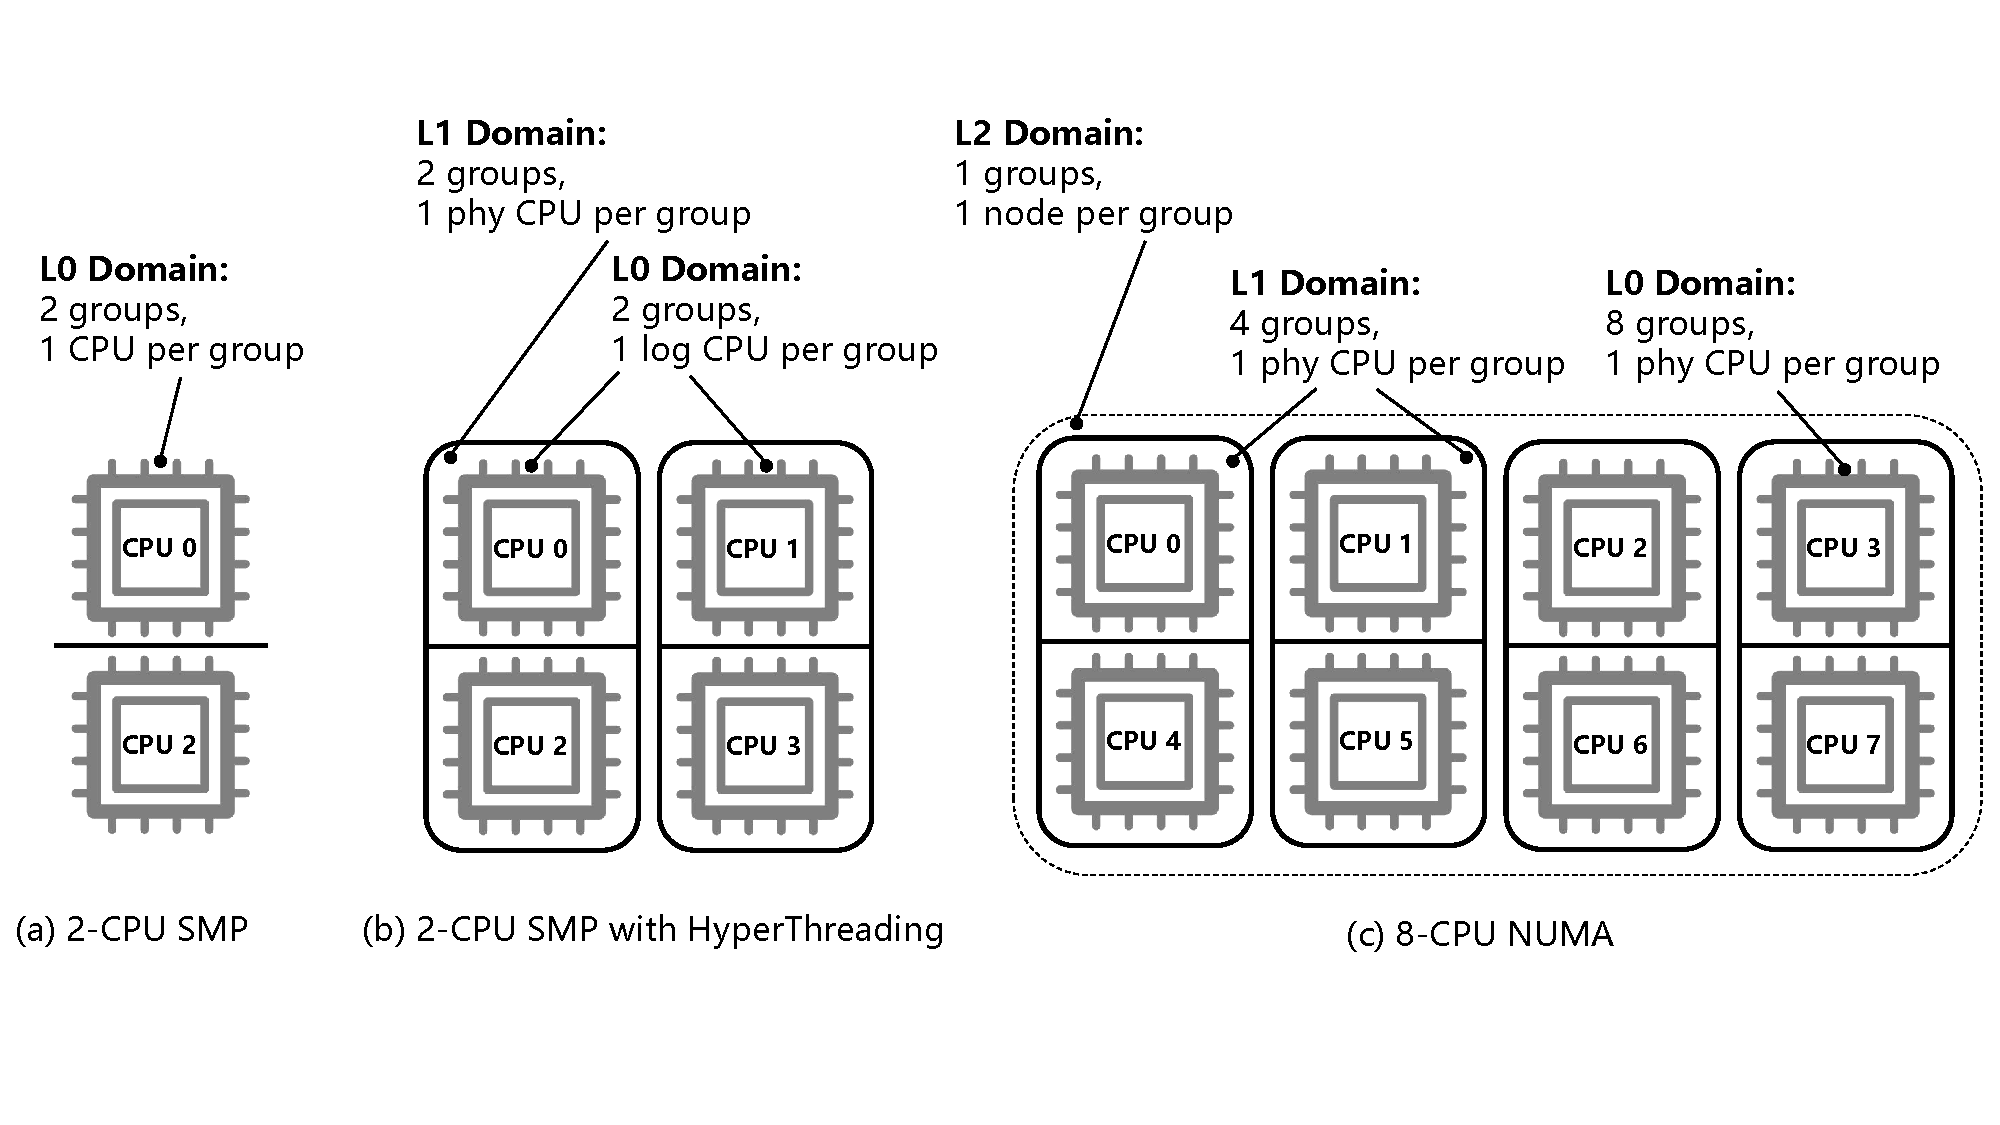
\includegraphics[width=1.0\textwidth]{scheduling_domain}
    \bicaption{\quad 调度域层级}{\quad scheduling domain hierachies}
    \label{fig:scheduling_domain}
\end{figure}

调度域充分反映了围绕CPU的共享资源信息信息。如表~\ref{tab:resourcesharing}所示,一个逻辑核通常是最底层的调度域,在这层调度域中,任务通过分时复用共享CPU资源,所有任务组织在一个或数个任务队列中,某一时刻仅有一个任务在运行,彼此几乎不存在影响。超线程组是更高一层的调度域,超线程技术由Intel公司提出,并最早于2002年引入市场,其通过增加CPU中的部分单元,使得能够在一个物理核心上虚拟出两个甚至多个逻辑核心,这些逻辑核心有自己的寄存器组与中断控制器,但彼此共享了执行单元、Cache和总线,这也意味着在这层调度域中运行的任务,彼此在这些资源上会产生竞争。现代采用NUMA架构的服务器中还有更高一层的NUMA调度域,NUMA(非一致存储器访问)架构中允许有多个CPU模块,每个CPU模块可以包含多个CPU,这些CPU拥有自己的本地内存与IO接口,彼此之间的通信交互通过互联模块完成,在这个调度域中,任务共享了相同的内存总线与LLC,同时在IO上也会彼此竞争。

\begin{table}
    \bicaption{\quad 调度域与共享资源}{\quad scheduler domains and resource sharing}% caption
    \label{tab:resourcesharing}
    \footnotesize% fontsize
    \setlength{\tabcolsep}{4pt}% column separation
    \renewcommand{\arraystretch}{1.5}% row space 
    \centering
    \begin{tabular}{lc}
        \hline
        %\multicolumn{num_of_cols_to_merge}{alignment}{contents} \\
        %\cline{i-j}% partial hline from column i to column j
        调度域 & 共享资源\\
        \hline
        Core & 几乎隔离\\
        HyperThread & 执行单元、缓存、总线\\
        NUMA & 末级缓存、内存带宽、IO\\
        \hline
    \end{tabular}
\end{table}

混部场景下QoS保障技术相关研究通常从三个方向展开:

1)其一是利用可观测性技术来进行应用性能画像与劣化监测。一方面是云厂商通过增强可观测性基础设施,来提升对数据中心持续监控与性能预警能力,2011年,Google公开了其数据中心混部集群监控数据集,国内阿里也在2017年公开了一部分混部集群的监控数据集\citep{guo2019limits},这些来自实际生产环境的脱敏数据集,极大促进了相关混部研究的发展。另一方面随云原生时代到来,可观测性粒度能细化到单个应用甚至函数,而通过对应用进行全面深入地观测,就能够利用丰富的指标数据来进行细致地画像分析,从而挖掘出更多的混部机会,制定更优的混部策略。

2)其二是围绕资源隔离的混部研究。资源隔离即通过软硬件等手段,强化混部场景下竞争应用在资源上的隔离性,防止因关键资源的竞争所引发的性能劣化。在软件上,可以通过Cgroup等手段配置任务的CPU亲和性,将彼此竞争的应用放置到不同的调度域中,也可以通过 traffic control技术\citep{hubert2002linux}协调任务对于网络资源的使用。在硬件上,可以采用Intel RDT技术\citep{guide2011intel},来对同一NUMA调度域中,共享末级缓存与内存带宽的任务进行资源协调,避免“吵闹邻居”问题\citep{xu2018dcat, maricq2018taming, rzadca2020autopilot, kwon2020dc}。

3)其三则尝试通过任务调度来解决干扰问题。基于资源划分的混部技术通常受限于软硬件的隔离能力,如Intel MBA对内存的调控就存在一定的延时\citep{herdrich2016cache},在瞬时流量激增的场景中就难以及时响应任务的资源需求。任务切换则能做到微秒级,同时资源的分配一般都以CPU分配为起点,只有当任务分配到CPU执行时,才会有后续其他资源的分配或使用。因此基于任务调度的研究一方面采用集中式队列来更好地进行全局调度决策,另一方面通过实施微秒级调度,让任务能够在短时间内获取CPU资源,从而减少延迟问题。

基于上述研究,本文首先设计了一套细粒度的可观测性系统,监测应用的性能指标并在其获取系统关键资源的路径上进行探测,完成对典型应用的画像分析。然后,本文提出了 Control Zone, 一种面向混部场景的分层可变调度系统,系统中首先按照CPU以及其他资源的拓扑,将服务器资源切割成数个隔离域,随后在隔离域中部署混部方案。而考虑到数据中心的混部方案随应用数量和画像的程度而增加,同时无论是围绕资源分配还是任务调度的混部手段,都无法保障能在每个场景下有效,Control Zone允许在不同隔离域中实施不同的内核调度策略,同时考虑到应用在不同负载下性能表现的不同,允许运行时对内核调度策略进行动态修改来适应混部策略的变化。而在隔离域外,则结合软硬件手段,来对影响任务性能的关键软硬件资源进行隔离保护。最后则针对不同的混部方案,设计一系列调度策略,提供常见混部场景的解决方案。

\section{国内外相关研究}

% 可观测性技术用来进行应用画像与劣化监测
% - 谁和谁能够混部
%   - 人为优先级: 延迟(LC/BE)
%   - 资源使用倾向/敏感度
% - 目标应用是否出现性能劣化/资源极限
% 调度技术的划分方式:
% - 实质: 
%   - CPU数量远小于任务数量时, 分时复用是常态,调度主要面向任务切换
%   - CPU数量足够时,任务可以并行,此时资源(异构CPU\Cache\Memory\IO\Net)共享是常态,因此调度主要面向资源划分
% - 任务切换: 修改或定制任务切换的逻辑,通过分时复用来实现共享资源的假象
%   - 实质是创建时间隔离域,来规避竞争
%   - 切换粒度与调度效果强相关, 能否及时响应任务的调度需求是设计的目标
% - 资源划分: 对任务使用的资源进行限制
%    - 创建资源隔离域,来规避竞争
%   - 任务仍在运行|任务由内核进行调度|不干涉任务调度过程
% 调度策略的划分方式:
% - 任务调度: 集中式、工作窃取、FIFO、CFS、EEVDF
% - 资源划分: 资源拆借

\subsection{数据中心可观测性与劣化监测研究现状}

%劣化监测
%分布式追踪(简单提一下)

SLO(Service-level objective)服务级别目标指定了用户所购买云服务功能的期望状态,通常包含服务可用性、带宽等基础指标,也包括每秒请求数量、尾延迟等业务性能指标。云厂商通过与用户协商SLO来定义云产品的质量保证,并在违反SLO时进行补偿。因此如何持续监测云服务质量并及时发现性能劣化时云厂商十分关注的问题。

可观测性技术是实现上述目标的基础设施,能够通过监控、日志记录、跟踪和其他数据收集手段来描述系统的状态,协助理解和诊断系统的行为和性能。大型数据中心中由于应用数量众多、软件环境复杂,因此云厂商更倾向于一些简单易懂的指标,来反映应用的性能,早期Google就使用CPI来作为应用的性能指标\citep{zhang2013cpi2}。CPI(Cycle Per Instruction)本身用于度量微观体系结构下的性能,应用正常运行时,CPI通常在一个小范围内波动,而当应用受到干扰导致运行速度变慢时,CPI的确能够很好地反映性能的劣化。然而在Li YI等人的研究中\citep{yi2020cpi},CPI在核心频率较低时存在较大的误差,并通过建模分析优化得到RCPI来对误差进行修正。

随AI技术的不断发展,研究者们发现数据中心的监控数据作为时序数据能够很方便地利用现有的AI数据分析技术进行分析,将AI和系统结合的研究也不断展开,而通过时序数据对服务性能劣化进行预测\citep{qiu2020firm, zhou2022aquatope, wang2022deepscaling, gan2021sage},也使得提前一步进行SLO保障成为可能。然而AI预测模型由于计算开销大、时间长,在单点调度上很难进行部署。

近年来随云原生可观测技术、DevOps技术的发展,可观测性技术在云服务中占据了越来越重要的地位。当前借助服务容器化以及容器编排技术的发展,云原生可观测性技术发展十分迅速。以指标监控为例,Prometheus监控系统提供了统一的数据采集格式以及灵活的检索系统\citep{brazil2018prometheus},而其在架构上的灵活性与可扩展性,也使得其能够方便地对大规模集群进行监控。而在服务质量上,2010年,Google提出了分布式追踪系统Dapper\citep{sigelman2010dapper},通过在rpc中嵌入span载荷,并允许span在rpc中进行传递,来实现对请求分布式处理过程的追踪。OpenTracing和OpenTelemetry等开源项目吸收了Dapper的核心思想并迅速在云原生社区中推广,当前大多数云原生应用都支持了基本的云原生可观测性,使得在集群中能够相对方便地收集云服务的QoS信息。同时,K8s向开发者开放了CNI(Container Network Interface)\citep{k8s-network-plugins},允许开发者自定义容器网络模型,同时能够结合eBPF、Envoy等云原生网络技术\citep{ebpf,envoyproxy},能够构筑一套完善Overlay Network系统,实现全链路的网络性能监测。

\begin{figure}[!htbp]
    \centering
    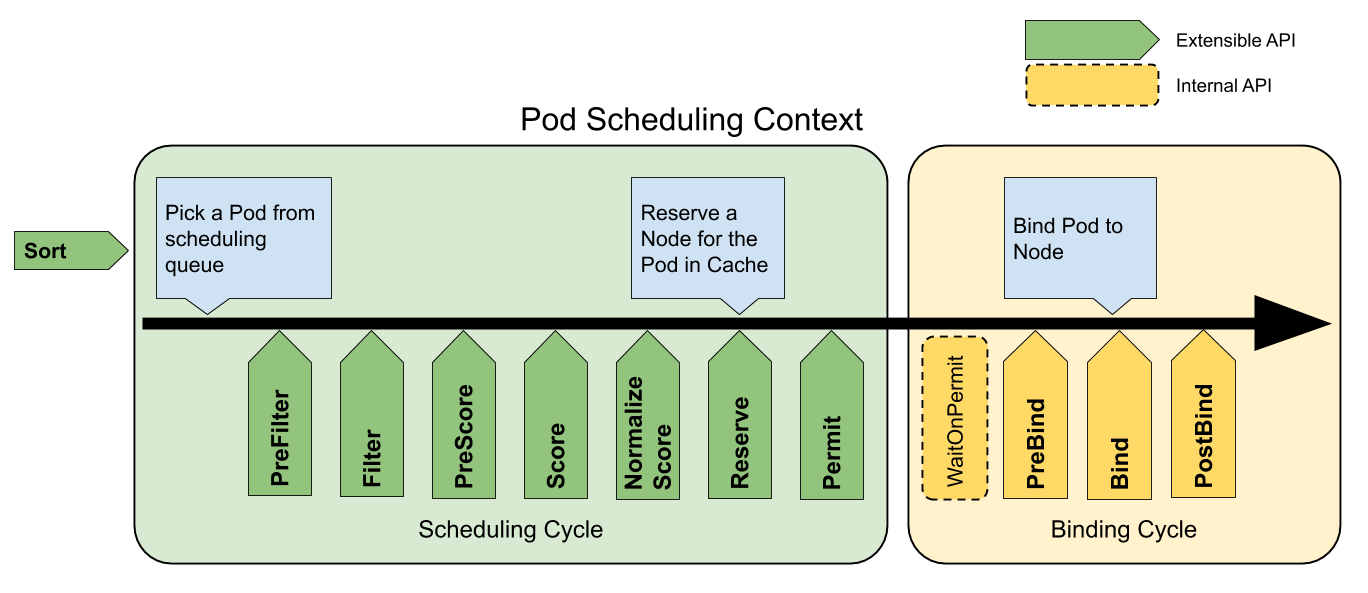
\includegraphics[width=0.85\textwidth]{k8s_scheduler}
    \bicaption{\quad k8s调度流程}{\quad k8s scheduler}
    \label{fig:k8s_scheduler}
\end{figure}

云原生可观测性地迅猛发展也提供丰富的监测信息,同时K8s所设计的基于标签的调度机制也极具灵活性(图~\ref{fig:k8s_scheduler}),而其为开发者提供了丰富的接口也大大降低了定制调度器的难度,以上这些都使得面向集群的劣化监测技术发展迅猛,其中FIRM\citep{qiu2020firm}就kubenetes集群为核心,设计了一种两级的机器学习模型来识别集群中服务性能劣化,在实验中取得了相当显著的效果。同时Di Wu\citep{wu2020data}则提出了一种数据特性感知潜在因素(DCALF)模型来实现高精度的QoS预测,能够依据不同QoS数据的特性来分别的进行预测。

\subsection{基于资源分配的SLO保障研究现状}

常规

细粒度

\subsection{基于任务调度的SLO保障研究现状}

Linux内核

微秒级调度

\section{论文的研究内容}

\subsection{典型应用画像与混部分析}

\subsection{运行时可变调度框架实现}

\subsection{资源感知调度系统实现}

\section{论文结构安排}
